\chapter{Implementation of Relational Operator}
\section{Assumption and Notation}

\subsection{Physical Data Organization}
\begin{itemize}
    \item Let us assume that each relation has attributes \textit{without null value}s, and it is stored in a heap file, or with the primary organization \textit{index sequential}.
    \item The indexes are organized as a B+–tree and those for non-key attributes are inverted indexes
    \item We also distinguish two types of indexes:
    \begin{itemize}
        \item A \textbf{clustered index} is built on one or more attributes of a relation sorted on the index key
        \item An \textbf{unclustered index} is built on one or more attributes which are not used to sort a relation
    \end{itemize}
\end{itemize}

\subsection{Physical Query Plan Operators}
\begin{tcolorbox}
The query optimizer has the task of determining how to execute a query in an “optimal” way, by considering the physical parameters involved. Each relational algebra operator can be implemented in different ways and the query optimizer must use appropriate strategies to estimate the costs of the alternatives and choose the one with lowest cost.
\end{tcolorbox}

\subsection{Physical Query Plan Execution}
Physical operators are implemented as \textit{iterators} that produce the records of the result one at a time on request. An iterator behaves as an \textit{object with state}, has a certain \textit{type}, can return the records in a certain order and has the following methods:
\begin{itemize}
    \item \textbf{open:} Initializes the process of getting records
    \item \textbf{isDone:} Tests if the iterator has more data to return
    \item \textbf{next:} Returns the next result record
    \item \textbf{reset:} Re-initializes the iterator already open
    \item \textbf{close:} Performs some clean-up operations and ends the iterator
\end{itemize}

Physical operators are either \textit{blocking} or \textit{non-blocking}. A blocking operator, when is opened, must call next exhaustively on its operands before returning its first (or next) record (e.g. the sort operator)

\section{Physical Operators for Relation $R$}
The records of a relation can be retrieved with any of the following operators, which have a relation R as an argument.
\begin{itemize}
    \item \textbf{TableScan($R$)} The operator returns the records of R, in the order that they are stored
    $$C=N_{pag}(R)$$
    \item \textbf{SortScan($R,\{A_i\}$)} 
    \begin{itemize}
        \item The operator returns the records of R sorted in ascending order on the set of attributes {Ai} values
        \item Sorting is done with the \textbf{merge sort} algorithm
        \item The operator’s cost depends on the $N_{pag}(R)$ value, the number of pages $B$ available in the buffer and the implementation of the \textit{merge sort}
        \item If the merge sort is implemented so that it returns the final result of the merge without first writing it to a temporary file, the cost will be more or less:
    \end{itemize}
    $$N_{pag}(R) = B \times (B-1)$$
    \item \textbf{IndexScan(R, $I$)}
    \begin{itemize}
        \item The operator returns the records of R sorted in ascending order on the set of attributes \{$A_i$\}
        \item Cost that depends on the type of index and the type of attribute on which it is defined.
        \[
        C = 
        \begin{cases}
        N_{leaf}(I) + N_{pag}(R) & \mbox{if } I\mbox{ is clustered} \\
        N_{leaf}(I) + N_{rec}(R) & \mbox{if } I\mbox{ is unclustered} \\
        N_{leaf}(I) + \lceil N_{key}(I) \times \Phi (\lceil N_{rec}(R)/N_{key}(I)\rceil, N_{pag}(R))\rceil & \mbox{if } I\mbox{ is an inverted index} 
        \end{cases}
        \]
        \end{itemize}
    \item \textbf{IndexSequentialScan(R,$I$)}
    \begin{itemize}
        \item The operator returns the records of $R$, stored with the primary organization \textit{index sequential} $I$
        \item Sorted in ascending order on the primary key values
        $$C = N_{leaf}(I)$$
    \end{itemize}
\end{itemize}

\section{Physical Operator for Projection $\pi^b$}
The physical operator that implements \textbf{projection}, without duplicate elimination, has as first argument the records returned by $O$, another physical operator.
\begin{itemize}
    \item \textbf{Project($O,\{A_I\}$)}
    \begin{itemize}
        \item The operator returns the records of the projection of the records of O over the set of attributes $\{A_i\}$
        \item No cost a part of the computational cost that can be ignored
        $$C = C(O)$$
    \end{itemize}
    \item \textbf{IndexOnlyScan($R,I,\{A_i\}$)}
    \begin{itemize}
        \item Return the sorted record over the projection to only a specific set of attributes using sorted index $I$ of the relative attributes $\{A_i\}$
        \item Usage of index since they are less heavy than records
        $$C = N_{leaf}(I)$$
    \end{itemize}
\end{itemize}

\section{Physical Operators for Duplicate Elimination $\delta$}
The  physical operators for \textbf{duplicate elimination} have as argument the records returned by $O$, another physical operator.
\begin{itemize}
    \item \textbf{Distinc($O$)}
    \begin{itemize}
        \item The records of $O$ must be \textit{sorted} so that duplicates will be next to each other
        \item Returns the records of O sorted, without duplicates
        $$C = C(O)$$
    \end{itemize}
    \item \textbf{HashDistinc($O$)}
    \begin{itemize}
        \item Returns the records of $O$ without duplicates using a hash technique
        \item We have $B + 1$ pages in the buffer to perform the duplicate elimination. Composed in two phases each one has a specific hash function
        \begin{itemize}
            \item $h_1$ - \textit{partitioning phase:} for each record of $O$ the hash function $h_1$ is used to distribute all the records uniformly in the $B$ pages. When a page is full it is written in the respective partition file. At the end we have a partition of the records of $O$ in $B$ files, each containing a collection of records that share a common hash value
            \item $h_2$ - \textit{duplicate elimination phase:} each partition is read page-by-page to eliminate duplicates with the hash function $h_2$ applied to all record attributes. A record $r$ is discarded only when it collides with another record $r'$ with respect $h_2$
        \end{itemize}
        $$C = C(O) + 2 \times N_{pag}(O)$$
        \item Same cost of distinct with the sorting of the operand records
        \item Disadvantage of not producing a sorted result
    \end{itemize}
\end{itemize}

\section{Physical Operators for Selection $\sigma$}
\begin{itemize}
    \item \textbf{Filter($O, \psi$)}
    \begin{itemize}
        \item Returns the records of $O$ satisfying the condition $\psi$ without indexes
        $$C = C(O)$$
    \end{itemize}
    \item \textbf{IndexFilter($R,I,\psi$)}
    \begin{itemize}
        \item Returns the records of $R$ satisfying the condition $\psi$ with the use of the index $I$
        \item The result will be sorted
        \item The operator is composed on two phases:
        \begin{itemize}
            \item It uses the index to find the sorted set of RIDs of the records satisfying the condition: RIDIndexFilter($I, \psi$)
            \item Retrieves the records of R: TableAccess($O, R$)
        \end{itemize}
        $$C = C_I + C_D$$
    \end{itemize}
    \item \textbf{IndexSequentialFilter($R,I, \psi$)}
    \begin{itemize}
        \item Returns the sorted records of R, stored with an \textbf{index sequential I} satisfying the condition $\psi$
        $$C = \lceil s_f(\psi) \times N_{leaf}(I)$$
    \end{itemize}
    \item \textbf{IndexOnlyFilter($R,I\{A_i\}, \psi$)}
    \begin{itemize}
        \item Return the sorted records of a selection with projection using only the index $I$
        $$C = \lceil s_f(\psi) \times N_{leaf}(I)$$
    \end{itemize}
    \item \textbf{OrIndexFilter($R, \{I_i, \psi_i\}$)}
    \begin{itemize}
        \item returns the records of R satisfying the \textit{disjunctive} condition: $\psi = \psi_1 \lor \psi_2 \lor ... \lor \psi_n$ using all the indexes $I_i$ one for each term $\psi_i$
        \begin{enumerate}
            \item Uses the indexes to find a sorted union of the RID list matching each terms $\psi_i$
            \item Return the records of $R$
        \end{enumerate}
        $$C_I = \Bigg \lceil \sum_{k=1}^n C_I^k \Bigg \rceil$$
        $$E_{rec} = \lceil s_f(\psi)\times N_{rec}(R)$$
        $$C_D= \lceil \Phi(E_{rec}, N_{pag(R)})\rceil$$
    \end{itemize}
    \item \textbf{AndIndexFilter($R, \{I_i, \psi_i\}$)}
    \begin{itemize}
        \item returns the records of R satisfying the \textit{conjunctive} condition: $\psi = \psi_1 \land \psi_2 \land ... \land \psi_n$ using all the indexes $I_i$ one for each term $\psi_i$
        \begin{enumerate}
            \item Uses the indexes to find a sorted intersection of the RID list matching each terms $\psi_i$
            \item Return the records of $R$
        \end{enumerate}
        $$C_I = \Bigg \lceil \sum_{k=1}^n C_I^k \Bigg \rceil$$
        $$E_{rec} = \lceil s_f(\psi)\times N_{rec}(R)$$
        $$C_D= \lceil \Phi(E_{rec}, N_{pag(R)})\rceil$$
    \end{itemize}
\end{itemize}

\section{Physical Operators for Grouping $\gamma$}
The records of R are partitioned according to their values in one set of attributes $\{A_i\}$ called \textit{grouping attributes}. Then, for each group, the values in certain other attributes are aggregated with the functions $\{f_i\}$.

\begin{itemize}
    \item \textbf{GroupBy($O,\{A_i\}, \{f_i\}$)}
    \begin{itemize}
        \item To group the records of $O$ on the set of attributes $\{A_i\}$ using the aggregation function in $\{f_i\}$
        \item In the set $\{f_i\}$ there are the aggregation function present in the SELECT and HAVING clauses
        \item The records of $O$ are sorted on the $\{A_i\}$
        $$C = C(O)$$
    \end{itemize}
    
    \item \textbf{HashGroupBy($O, \{A_i\}, \{f_i\}$)}
    \begin{itemize}
        \item The records of $O$ are partitioned using a hash function on the attributes $\{A_i\}$
        \item Two phases:
        \begin{enumerate}
            \item \textit{partitioning phase:} a partition is created using the hash function $h_1$
            \item \textit{grouping phase:} the records of each partition are grouped with the hash function $h_2$
        \end{enumerate}
        $$C = C(O) + 2 \times N_{pag}(O)$$
    \end{itemize}
\end{itemize}

\section{Physical Operators for Join $\bowtie$}
The cartesian product plus the filter create all possible tuple and remove all pairs that doesn't match the foreign key, but this is not efficient.

We will consider the equijion computed with one of the following physical operators, where:
\begin{itemize}
    \item $O_E$ is the external operand
    \item $O_I$ is the internal operand
    \item $\psi_I$ is the join condition
\end{itemize}
\begin{itemize}
    \item \textbf{NestedLoop($O_E, O_I, \psi_J$)}
    \begin{figure}[h]
        \centering
        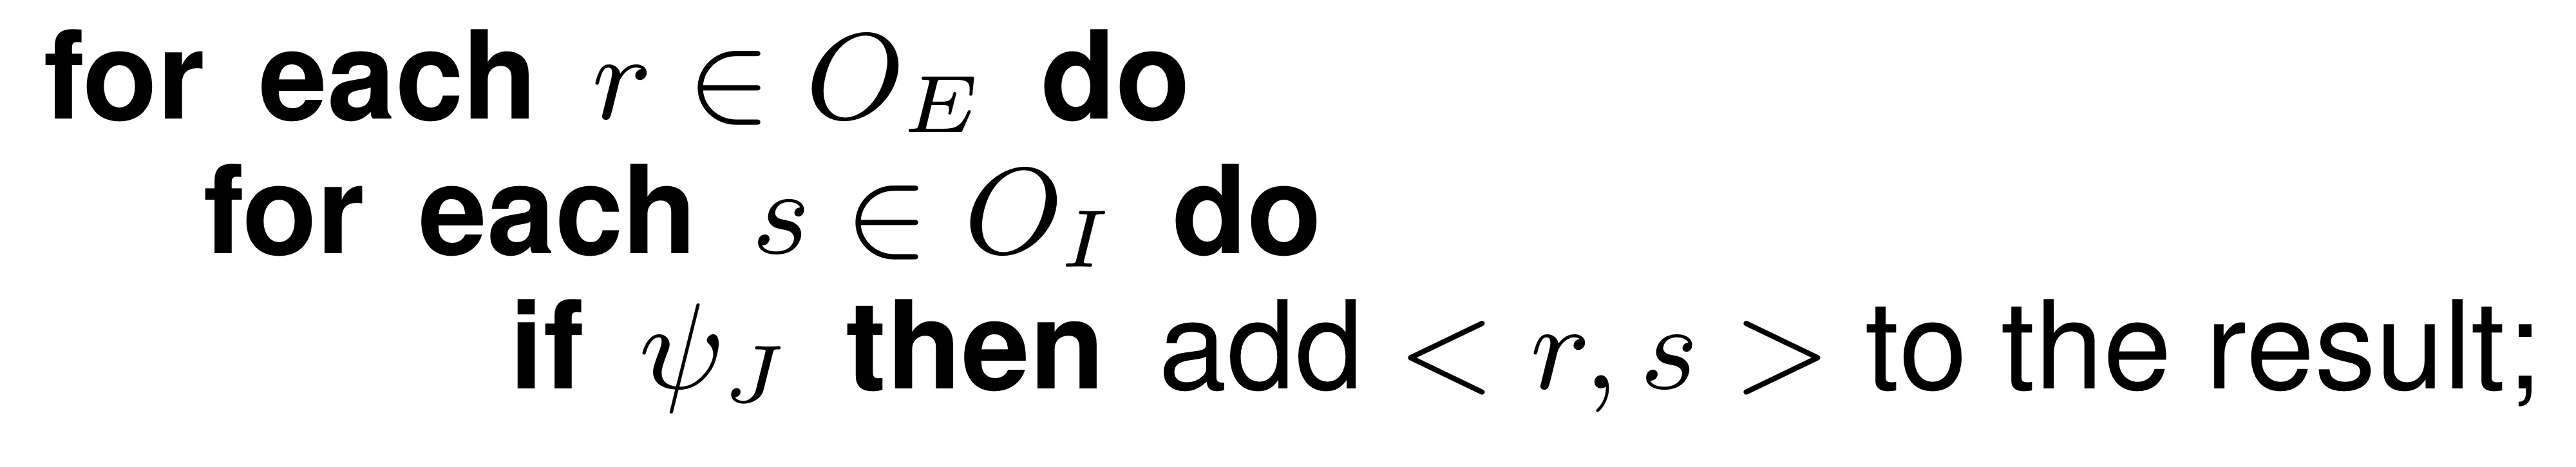
\includegraphics[width=.5\linewidth]{images/DBMS_Internals/ImplementationOfRelationalOperator/NestedLoop.jpeg}
        \end{figure}
    \begin{itemize}
        \item It verify if every possible pair satisfy the predicate $\psi$
    \end{itemize}
    $$C_{NL} = C(O_E) + E_{rec(O_E) \times C(O_I)}$$
    \item \textbf{PageNestedLoop($O_E, O_I, \psi_J$)}
    \begin{itemize}
        \item The cost of the nested loop join can be reduced considerably if, instead of scanning the result of $O_I$ once per record of $O_E$, we scan it once per page of $O_E$
        \item The inner relation is scanned only once for page of the puter relation
        
        $$C_{PNL} = C(O_E) + N_{pag}(O_E) \times C(O_I)$$
        $$C_{PNL} = N_{pag}(S) + N_{pag}(S) \times N_{pag}(R)$$
        \item This method is better than the NestedLoop since $N_{pag}(R) < N_{rec}(R)$, but it has the defect of producing an unsorted result

        \begin{figure}[h]
        \centering
        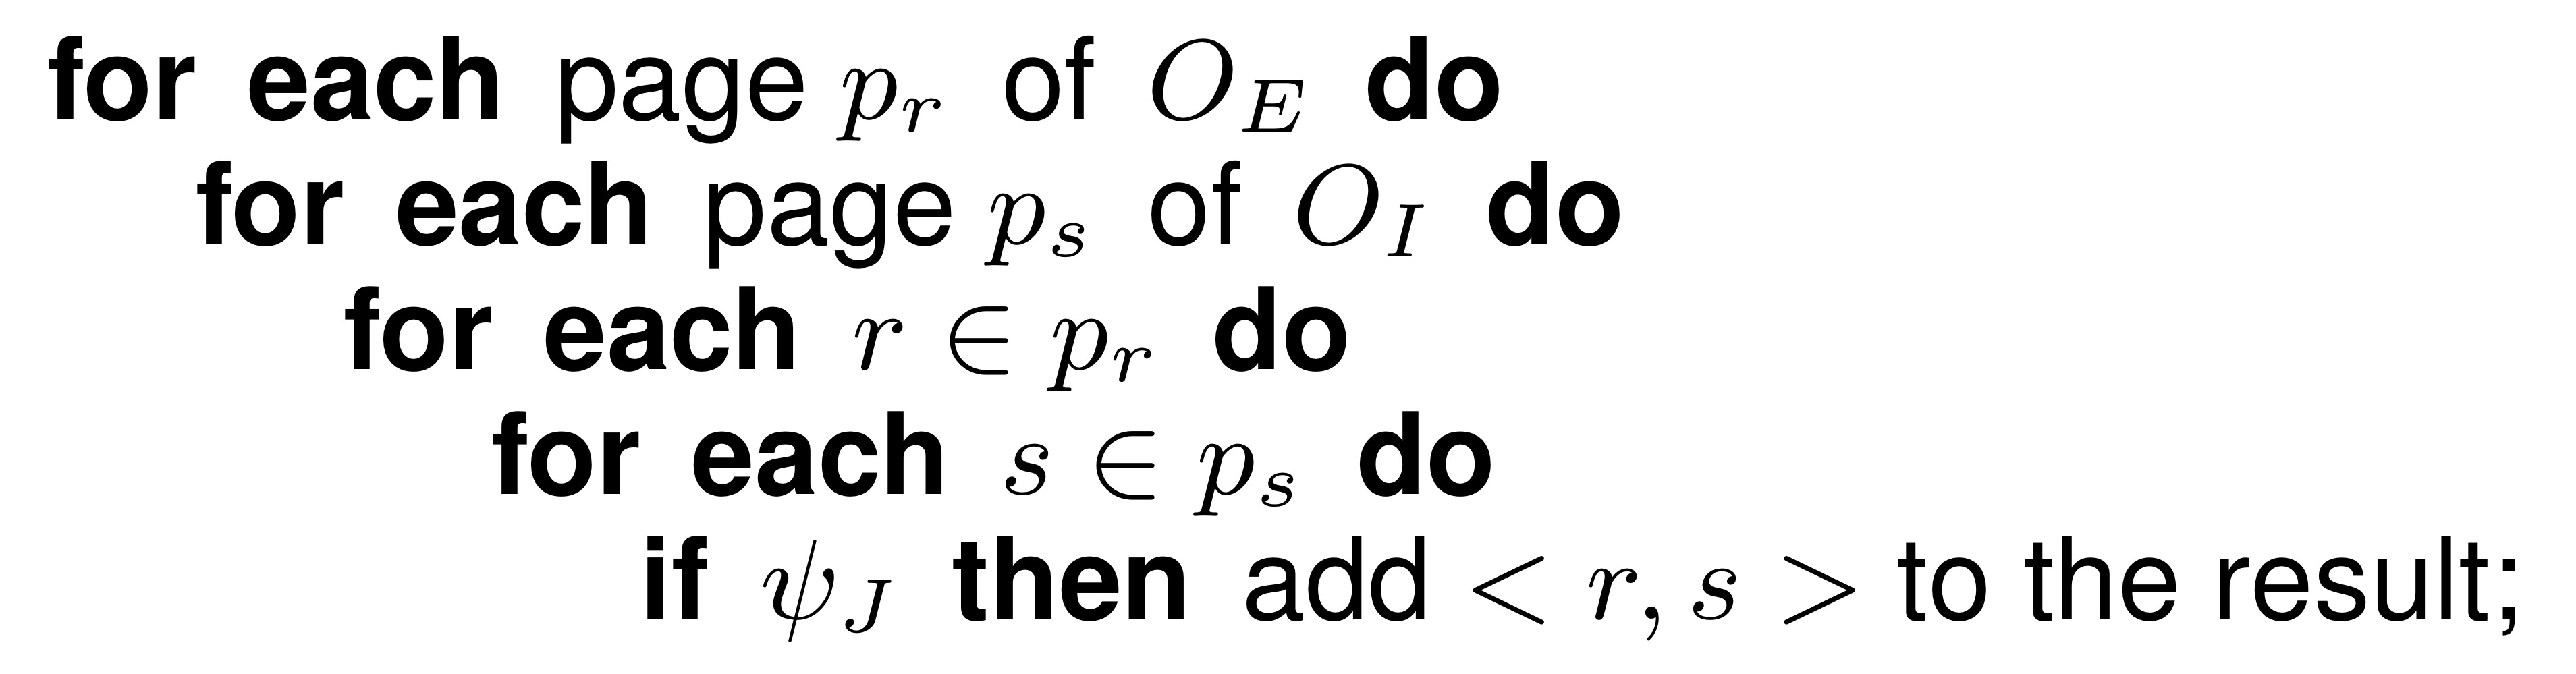
\includegraphics[width=.5\linewidth]{images/DBMS_Internals/ImplementationOfRelationalOperator/PageNestedLoop.jpeg}
        \end{figure}
    \end{itemize}
    
    
    \item \textbf{IndexNestedLoop($O_E, O_I, \psi_J$)}
    \begin{itemize}
        \item Only with \textit{equi-join}
        \item In case there is an index on the join column of one relation, we can exploit it
        \item Still goes through the external operator
        \item Use the index to restrict the search, no need to check the condition since it is already satisfied
        \begin{figure}[h]
        \centering
        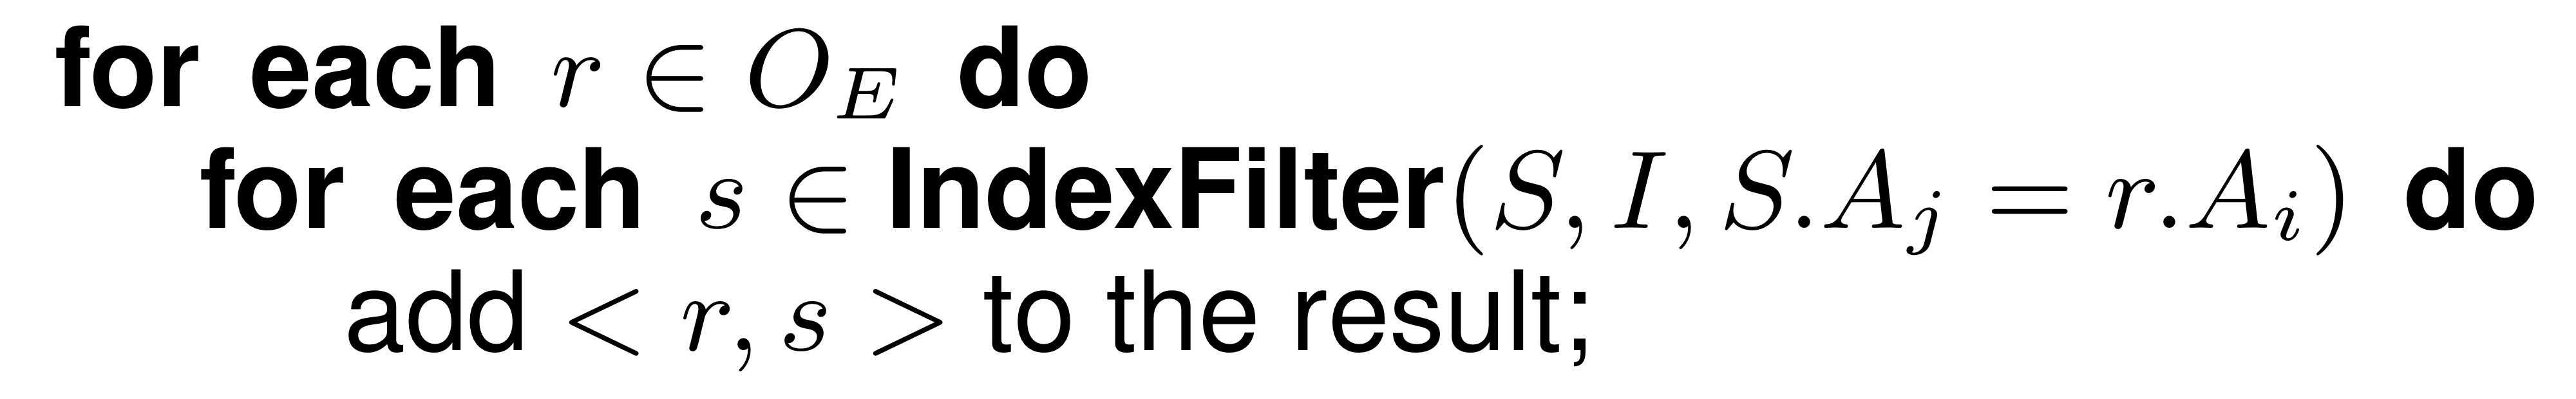
\includegraphics[width=.5\linewidth]{images/DBMS_Internals/ImplementationOfRelationalOperator/IndexNestedLoop.jpeg}
        \end{figure}
        $$C_{INL} = C(O_E) + E_{rec}(O_E) \times (C_I + C_D)$$
        \item $(C_I + C_D)$ is the cost to retrieve the matching records of S with a record of $O_E$ that depends on the index type
    \end{itemize}

    \item \textbf{MegeJoin($O_E, O_I, \psi_J$)}
    \begin{itemize}
        \item Only with \textit{equi-join} plus sort-merge
        \item $O_E$ and $O_I$ records are \textit{sorted} on the join attributes columns
        \item The $O_E$ join attribute is a key
        \item Join attribute is a key
        $$C_{MJ} = C(O_E) + C(O_I)$$
    \end{itemize}
    
    \item \textbf{HashJoin($O_E,O_I,\psi_J$)}
    \begin{itemize}
        \item In case we do not have sorted data we can use two distinct hash functions in two phases in order to compute the join
        \begin{enumerate}
            \item \textit{partitioning phase:} the records of $O_E$ and $O_I$ are partitioned using the function $h_1$
            $$C(O_E) + C(O_I) + N_{pag}(O_E) + N_{pag}(O_I)$$
            \item \textit{probing phase:}
            \begin{itemize}
                \item For each partition the records of $O_E$ are read and inserted into the buffer hash table with B pages using the function $B$
                \item The records of $O_I$ are read one page at a time and the one joining with $O_E$ are checked with $h_2$
                \item And added to the result
            \end{itemize}
            $$N_{pag}(O_E) + N_{pag}(O_I)$$
        \end{enumerate}
        \item The total cost is:
        $$C_{HJ} = C(O_E) + C(O_I) + 2 \times (N_{pag}(O_E) + N_{pag}(O_I))$$
    \end{itemize}
\end{itemize}

\section{Physical Operators for Set and Multiset Union, Intersection and Difference}
\textbf{Union($O_E, O_I$), Except($O_E, O_I$), Intersect($O_E, O_I$)}:
\begin{itemize}
    \item Require that the records of the operands are sorted and without duplicates
    \item The variants with \textbf{All} do note require to eliminate the duplicates
    \item The \textbf{UnionAll} is simple and powerful
    \item They all have cost equal to:
    $$C = C(O_E) + C(O_I)$$
\end{itemize} 
